\section{Coleta de Dados}

%===============================================
\subsection{Diponibilidade dos dados}

Falar como está disponibilidade das colunas 


%===============================================
\subsection{Visualização dos dados}

\tab
Caso deseja somente ler os dados da bancada a própria
ESP-IDF faz esse trabalho, basta aperta no ícone  de
monitor localizado na parte inferior da Janela do 
Visual Studio Code (Figura \ref{fig:Icones}).

\begin{figure}[!ht]
    \centering
    \caption{Ícone}
    \vspace{0.2cm}
    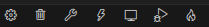
\includegraphics[scale=0.8]{img/icones.png}
    \label{fig:Icones}
\end{figure}

Aparecerá um terminal parecido como na Figura 
\ref{fig:Monitor} com uma mensagens de \textit{log}.
As colunas importantes são as que estão escritas em branco.

\begin{figure}[!ht]
    \centering
    \caption{Ícone}
    \vspace{0.2cm}
    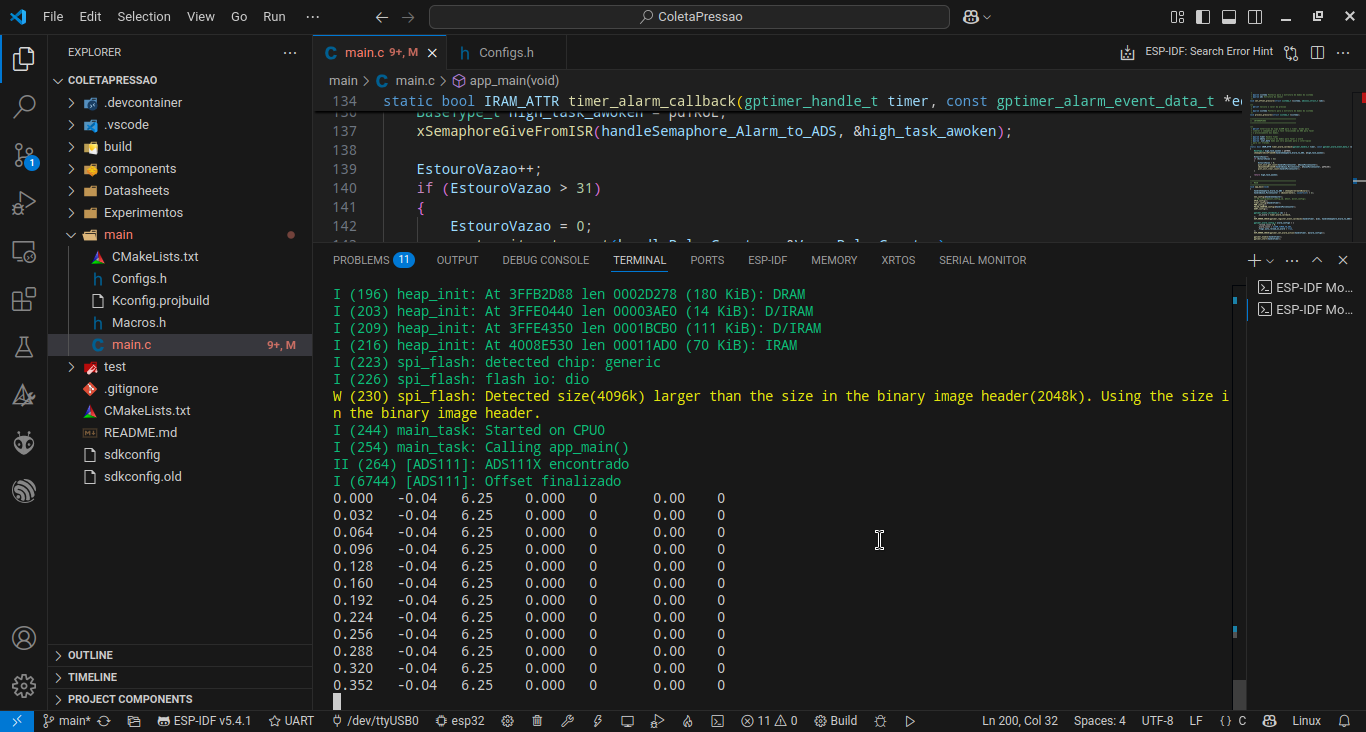
\includegraphics[scale=0.2]{img/TerminalDados.png}
    \label{fig:Monitor}
\end{figure}
